\documentclass[11pt, letterpaper]{report}
\usepackage{graphicx}
\usepackage{float}  % Needed for the 'H' specifier

% Ensure single spacing
\linespread{1}

\title{\textbf{Pokemon Rank Classifier}}
\author{\textbf{ECS 171 Machine Learning} \\\\Group Leader: Alex D'Souza \\ Group Members: Catherine Chen, Varun Wadhwa, Shane Kiim}
\date{\textbf{Github Repository: }https://github.com/AlexanderDsouza/ECS171GroupProject}

\begin{document}
    \maketitle
    \chapter{Introduction and background}
    In this project we found 

    \chapter{Literature Review}
    
    \chapter{Dataset Description}
  
    \begin{figure}[H]
        \centering
        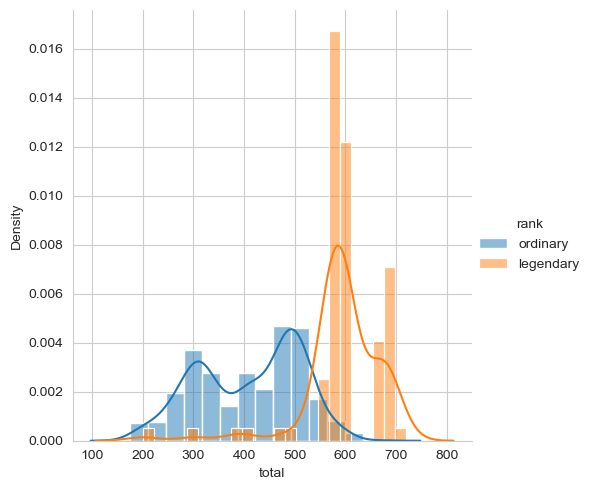
\includegraphics[width=0.8\textwidth]{histplot.png} % Adjust the width as needed
        \caption{Histogram of the Dataset}
        \label{fig:dataset-hist}
    \end{figure}
  This section provides a description of the dataset used in our study. To illustrate the characteristics of the dataset, we include a histogram plot shown in Figure \ref{fig:dataset-hist}. As you can see at around 550 in total stats, legendary Pokemon and ordinary Pokemon make a distinct split. When we saw this, we decided that a linear SVM model would be perfect for our dataset as you can clearly draw a line right in between that mark and it could split the classes pretty accurately. 

    \begin{figure}[H]
        \centering
        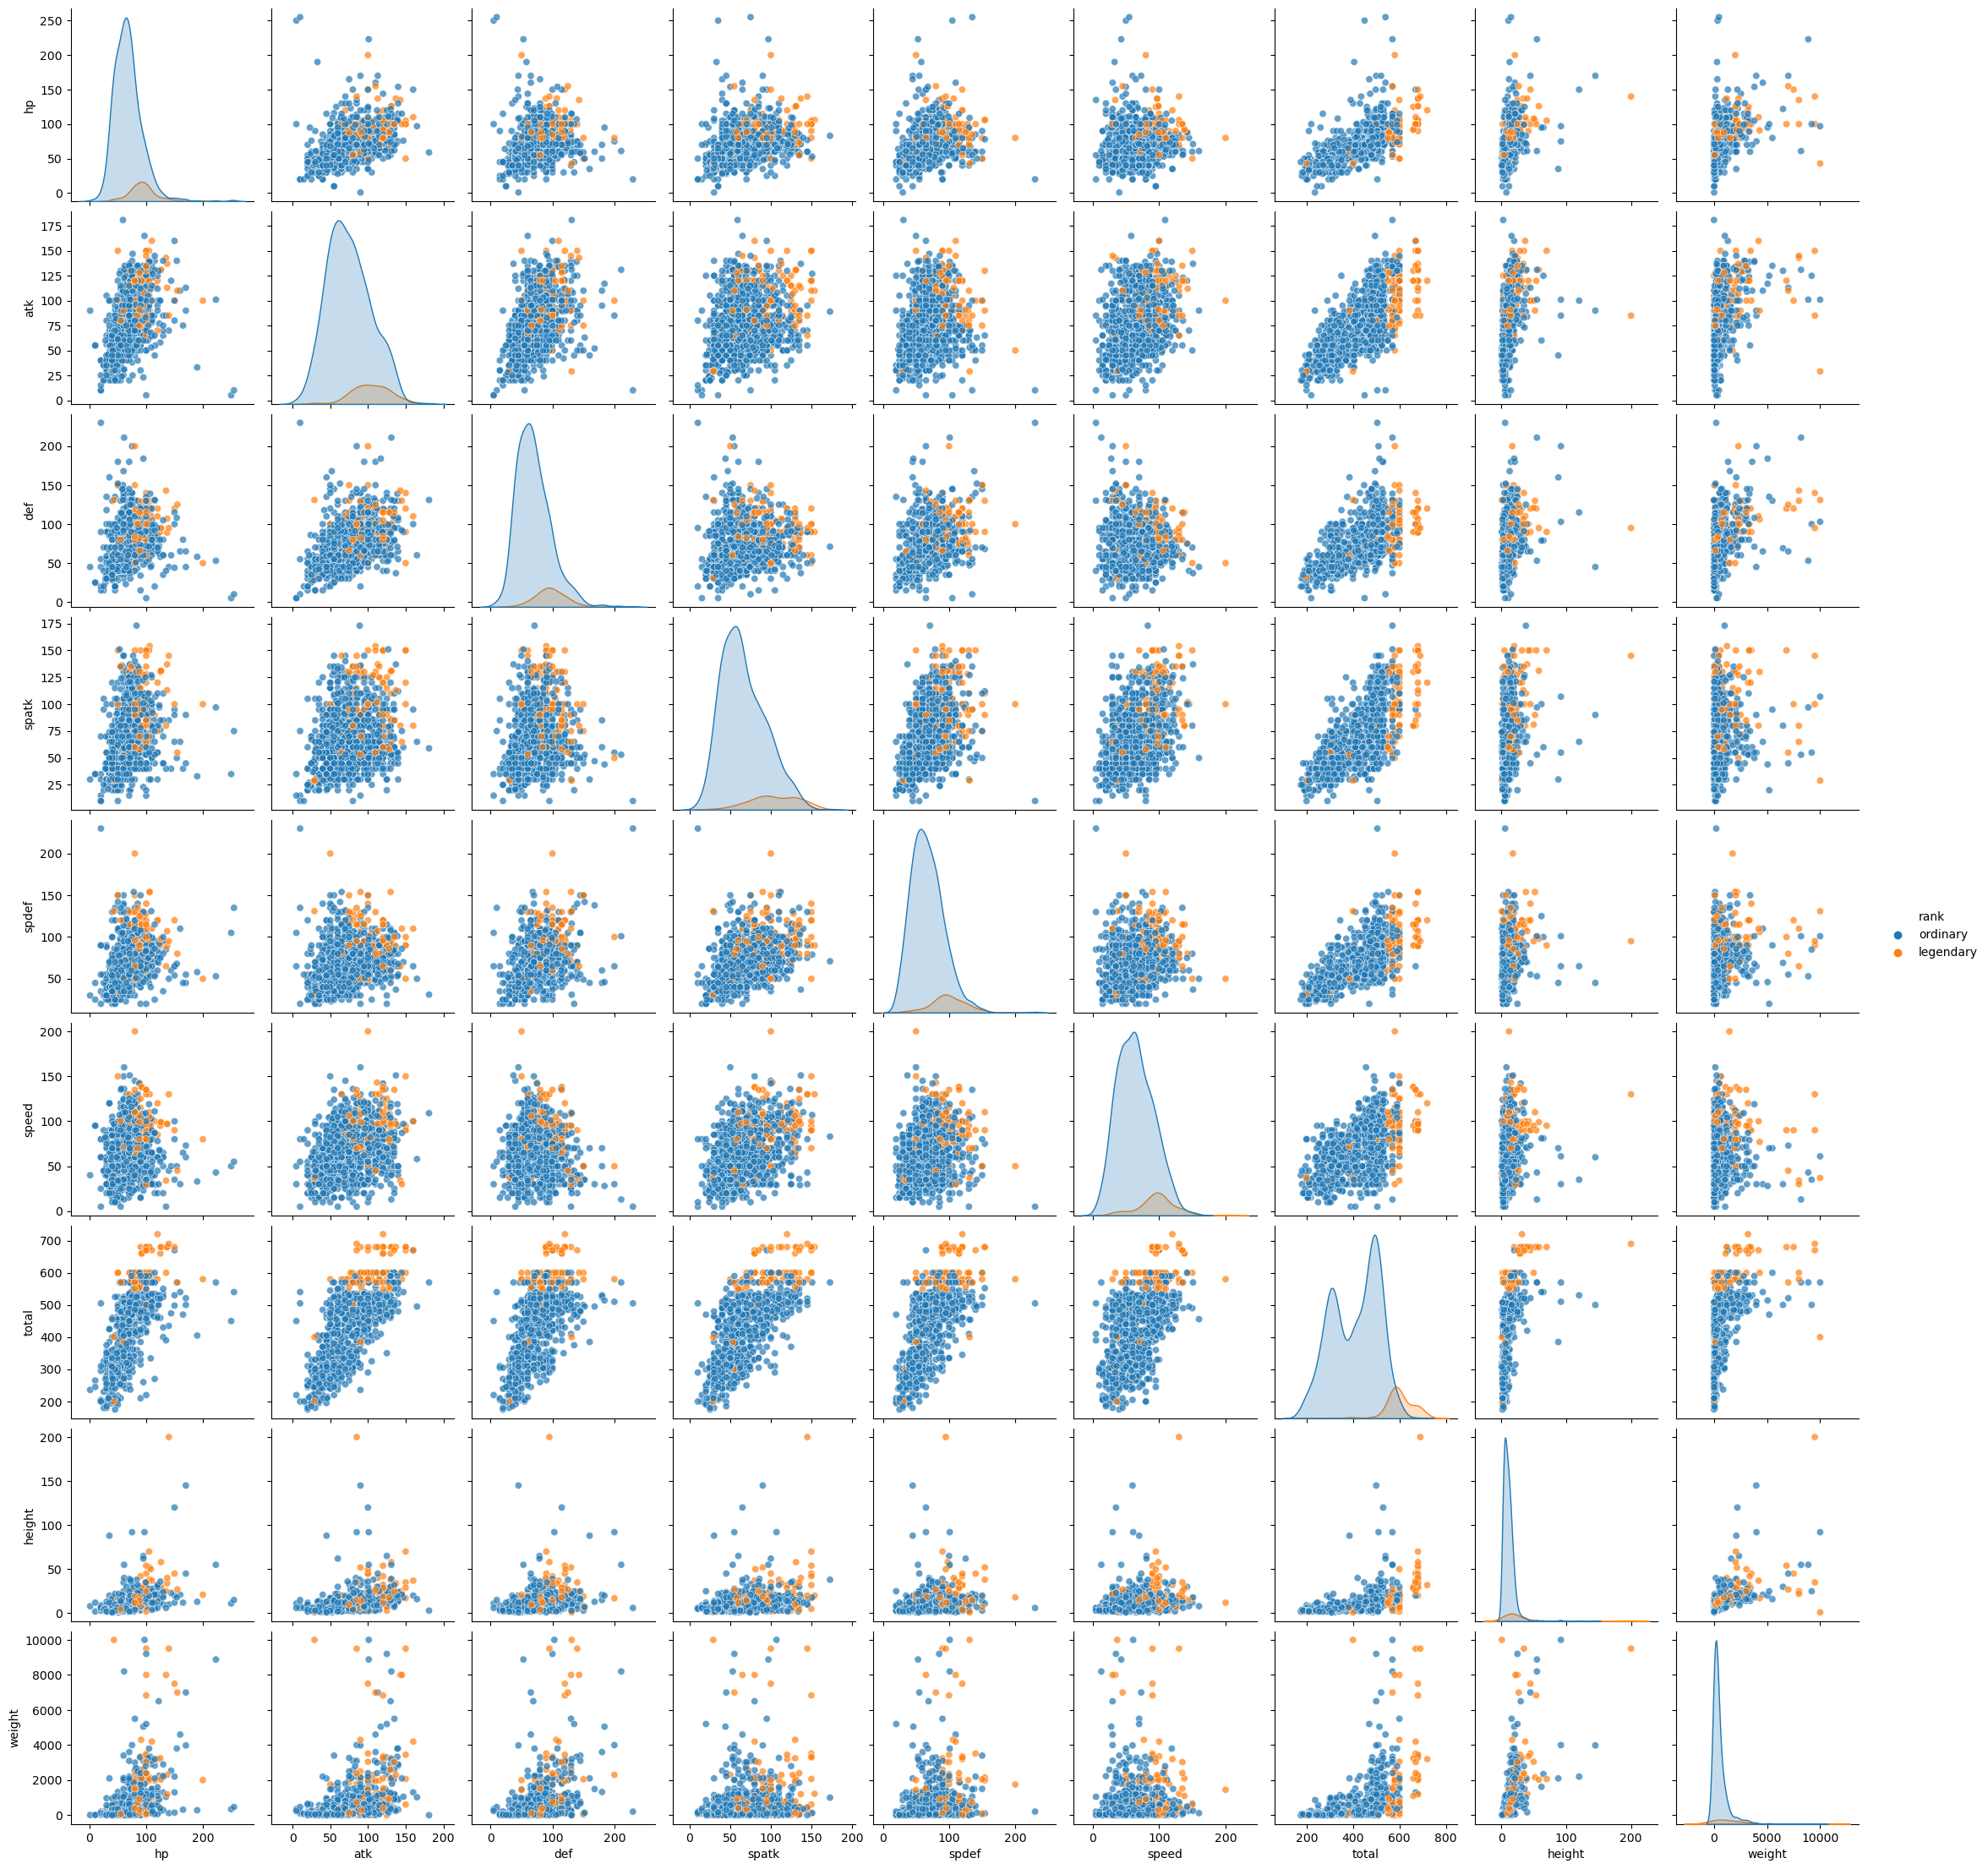
\includegraphics[width=0.8\textwidth]{pairplot.png} % Adjust the width as needed
        \caption{Pair Plot of the Dataset}
        \label{fig:dataset-pairplot}
    \end{figure}
In the pairplot we can also see that in the total pairplots, we can easily cut the classes and group them with a line. This also led us to believe SVM would be extremely good. 

    \chapter{Proposed Methodology}
    \chapter{Experimental Results}
    \chapter{Conclusion and Discussion}
    \chapter{References}
\end{document}
